
\documentclass[aps,prl,twocolumn,superscriptaddress]{revtex4-2}


\usepackage{graphicx}
\usepackage{epstopdf}

\usepackage{amssymb}
\usepackage{amsmath}
\usepackage{color}
\usepackage{hyperref}
\usepackage{tikz}
\usepackage{mathrsfs}
\usepackage{wasysym}
\usepackage{tikz-cd}
\usepackage{stackengine,scalerel}

\usepackage{float}

% Entorno español.
\usepackage[spanish]{babel}
\addto\captionsspanish{%
  \renewcommand{\tablename}{Tabla}%
  \renewcommand{\figurename}{Figura}%
}

% so sections, subsections, etc. become numerated.
\setcounter{secnumdepth}{3}

\DeclareMathOperator*{\argmax}{arg\,max}
\DeclareMathOperator*{\argmin}{arg\,min}
\newcommand{\avrg}[1]{\left\langle #1 \right\rangle}
\renewcommand{\appendixname}{Apéndice} % Change "Appendix" to "Apéndice"

\begin{document}

\title{
El modelo neuronal de Izhikevich
}

\author{Bianca Abril Petry}
\email[]{bianca.petry@mi.unc.edu.ar}
\affiliation{Facultad de Psicología, Universidad Nacional de Cordoba, Boulevard de la Reforma esq. Enfermera Gordillo Gómez, Ciudad Universitaria, Córdoba, Argentina.  }

\author{Alex Ivan Wicher}
\email[]{ivan.wicher.038@mi.unc.edu.ar}
\affiliation{Facultad de Matem\'atica, Astronom\'ia, F\'isica y Computaci\'on, Universidad Nacional de C\'ordoba, Ciudad Universitaria, 5000 C\'ordoba, Argentina}

\author{Arapayu Javier Alejandro}
\email[]{arapayujavier@gmail.com}
\affiliation{Facultad de Ciencias Exactas y Naturales y Agrimensura, Universidad Nacional del Nordeste, Av. Libertad 5460, Corrientes, Argentina.}


\date{\today}

\begin{abstract}
En este trabajo se implementa y analiza numéricamente el modelo de neurona de disparo bidimensional de Izhikevich para el estudio de la dinámica electrofisiologica neuronal. Utilizando el método de integración de Runge-Kutta de orden 4 (RK4) y una regla discreta de reseteo, se simula la evolución temporal del potencial de membrana $v{(t)}$ y la variable de recuperación $u{(t)}$ ante distintos estímulos de corriente $I{(t)}$. Los resultados obtenidos reproducen cualitativamente los ocho patrones principales de dinámica neuronal reportados en la literatura ({Regular Spiking, Intrinsically Bursting, Chattering, Fast Spiking, Low-Threshold Spiking, Thalamo-Cortical} en dos condiciones y Resonator ). Se discuten las propiedades dinámicas de cada régimen así como el impacto de las aproximaciones numéricas y la condición de reseteo en la estabilidad de las soluciones.


\end{abstract}

\maketitle

\section{Introducción}

Los modelos matemáticos de neuronas de disparo constituyen una herramienta esencial en neurociencia computacional para comprender cómo las células cerebrales procesan información mediante impulsos eléctricos. Históricamente, el diseño de estas simulaciones enfrenta un dilema fundamental entre dos requisitos excluyentes: la simplicidad computacional y la plausibilidad biológica. Por un lado, los modelos biofísicamente detallados de tipo Hodgkin y Huxley \cite{hodgkin1952quantitative}, describen con precisión la cinética iónica relevante \textit{spike} (Na, K) de los canales de membrana, pero su elevado costo computacional limita las simulaciones a solo un puñado de células en tiempo real. Por otro lado, los modelos tradicionales de integración y disparo (\textit{integrate-and-fire}) son computacionalmente eficientes, pero carecen de realismo biológico y son incapaces de reproducir la rica variedad de patrones de disparo y ráfagas (\textit{bursting}) de la corteza cerebral.

En este contexto, Izhikevich propuso un modelo reducido bidimensional derivado de la teoría de bifurcaciones y formas normales, extendiendo del que combina lo mejor de ambos enfoques: la baja carga computacional del \textit{integrate-and-fire} con la flexibilidad y el realismo biológico de Hodgkin-Huxley \cite{izhikevich2003simple}. El objetivo de este informe es implementar numéricamente dicho modelo mediante el algoritmo de Runge-Kutta 4 (RK4) con un paso temporal  $h = 0.1\text{ ms}$ , validar su respuesta inicial y reproducir cualitativamente los ocho comportamientos electrofisiológicos principales de neuronas corticales y talámicas.

\section{Teoría}

Corrientes sinápticas producen cambios, llamados potenciales post-sinápticos (\textit{PSPs}). Grandes corrientes producen significativos \textit{PSPs} que pueden ser amplificados por canales sensibles al voltaje en la membrana de la neurona que provocan la generación de potencial de acción, disparo o \textit{spike}. El método principal de comunicación de la neurona es el \textit{spike}.
Por eso ha sido de gran interés para entender como procesa información el cerebro modelar los factores electro-fisiológicos que inducen a una neurona al spike. Requerimos para escalar de una neurona a redes neuronales que estos modelos sean computacionalmente viables y biológicamente factibles a los comportamientos reales de los tipos relevantes de neuronas y sus comportamientos de disparo.
Un resultado importante de los experimentos de Hodgkin-Huxley es que las neuronas son sistemas dinámicos. En su modelo identificaron dos corrientes iónicas de sodio, potasio como las mas relevantes en la excitabilidad de neuronas, abstrayendo otras corrientes de perdida, representando el efecto agregado de estas corrientes abstraídas por el modelo.
Existen decenas de corrientes conocidas, puramente como argumento combinatorio implica que hay millones de diferentes mecanismos electro-fisiológicos de generación de \textit{spike}, pero solo hay cuatro tipos diferentes de bifurcación de equilibrio. En particular, nos interesa la bifurcación \textit{saddle-node} cuya forma normal es \textit{quadratic integrate and fire} $v=v^2+I$, siendo $I$ la corriente. Esta bifurcación ocurre cuando dos puntos de equilibrio de un sistema dinámico colisionan y desaparecen a medida que un parámetro (corriente) cambia. Cruzar esta bifurcación puede ocasionar que una neurona transaccione de un estado estable de descanso a una de disparo repetitivo \cite{izhikevich2007dynamical}.
El modelo de Izhikevich se formula mediante un sistema bidimensional de ecuaciones diferenciales ordinarias (\textit{EDOs}) no lineales:
\begin{align}
    \dot{v}(t) &= 0{,}04v^2(t) + 5v(t) + 140 - u(t) + I(t), \label{eq:izhi_v} \\
    \dot{u}(t) &= a (b v(t) - u(t)), \label{eq:izhi_u} 
\end{align}
acoplado a un mecanismo discreto de reseteo cuando el potencial alcanza o supera una cota superior:
\begin{equation}
    \text{si } v(t) \geq 30\text{ mV, entonces } 
    \begin{cases} 
        v(t) \leftarrow c \\ 
        u(t) \leftarrow u(t) + d 
    \end{cases} \label{eq:izhi_reset}
\end{equation}

Donde $v(t)$ representa el potencial de membrana de la neurona (en mV), $u(t)$ la variable de recuperación de membrana, la cual modela la activación de corrientes hacia afuera de potasio y la inactivación de corrientes de sodio, proveyendo realimentación negativa a $v(t)$, por último, $I(t)$ representa la corriente externa inyectada o la entrada sináptica efectiva.

Por su parte, los parámetros adimensionales $a, b, c, d$ cumplen las siguientes funciones:
\begin{itemize}
    \item $a$: determina la escala temporal de recuperación de la variable $u(t)$.
    \item $b$: define la sensibilidad de $u(t)$ ante fluctuaciones subumbrales de $v(t)$.
    \item $c$: fija el valor al que se resetea el potencial de membrana $v(t)$ tras un disparo (\textit{spike}).
    \item $d$: establece el incremento en la variable $u(t)$ provocado por el evento de disparo.
\end{itemize}
Los coeficientes específicos 0.04, 5, 140 definen una escala particular de voltaje y un \textit{offset}.
La condición $v(t) \geq 30\text{ mV}$ no constituye un umbral fisiológico fijo de disparo, sino un umbral de corte algorítmico utilizado por el programa para registrar la cima del \textit{spike} y aplicar el reseteo discreto. En este modelo, el inicio del disparo es una propiedad emergente y dinámica que depende del estado previo conjunto de las variables $v(t)$ y $u(t)$ \cite{izhikevich2007dynamical}.
En la realidad sucede algo como lo de la figura \ref{fig:fig0} 

\begin{figure}
    \centering
    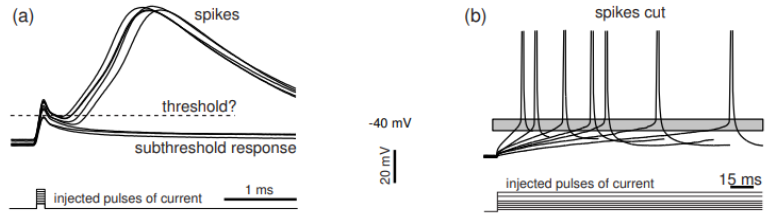
\includegraphics[width=1\linewidth]{ratsSpikes.png}
    \caption{El umbral de disparo no es discreto. Se observan dos grabaciones in vitro de neuronas de rata de la capa 5 de la corteza cerebral.\cite{izhikevich2007dynamical}}
    \label{fig:fig0}
\end{figure}

\section{Resultados}
Un modelo neuronal integrate and fire posee una dinámica de picos periodicos en el potencial de membrana, característicos en algunas neuronas biológicas como la RS (regular spiking) y la CH(chattering)(\cite{izhikevich2003simple}. El modelo matemático \eqref{eq:izhi_v}, \eqref{eq:izhi_u} exhibe una dinámica general como se muestra en la figura \ref{fig:fig1}, obtenida mediante integración numérica. En la figura se detalla el potencial de membrana $v$, la variable de recuperación $u$ y la corriente de entrada $I$ en función del tiempo. En en panel superior de la figura se observa el reposo submbral del potencial de membrana para $t < 10$ ms y la aparición de disparos periódicos tras la aplicación del estímulo en $t = 10$ ms (panel inferior), donde cada pico es llevado a $30$mV antes de aplicar el reseteo. Este modelo por lo tanto muestra una dinámica de picos regulares, así como los modelos más complejos, evidenciando utilidad del sistema \eqref{eq:izhi_v}, \eqref{eq:izhi_u}  como modelo neuronal. 
 

\begin{figure}
    \centering
    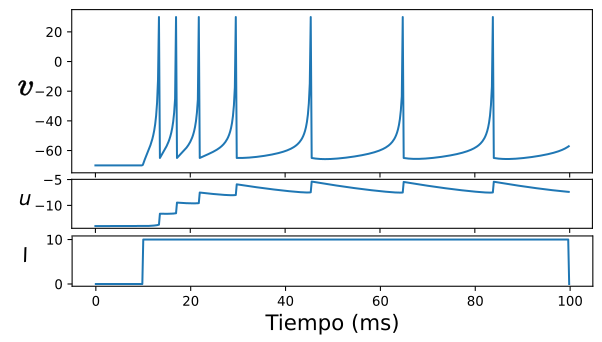
\includegraphics[width=0.88\linewidth]{figs/fig1.png}
    \caption{Evolución temporal del potencial de membrana ($v$), la variable de retardo ($u$) y el estimulo ($I$). Las distintas dinámicas se lograron siguiendo distintos protocolos y valores de parámetros del sistema dinámico (ver apéndice). }
    \label{fig:fig1}
\end{figure}

El modelo propuesto por Izhikevich resulta a su vez, capaz de reproducir en comportamiento dinámico de los potenciales de membrana de distintos tipos de neuronas.  Distintos comportamientos se logran mediante la configuración de los parámetros del sistema dinámico, además de un diseño especifico para la corriente de entrada $I(t)$ y de las condiciones iniciales de evolución $(v_0,u_0)$. 

En la figura \ref{fig:fig2} se presentan los resultados numéricos de evolucionar temporalmente la neurona de Izhikevich con configuraciones distintas (ver apéndice). Cada panel de la figura describe un patrón distinto de picos o de comportamiento subumbral:
\begin{itemize}
        \item \textbf{a) RS (}\textit{\textbf{Regular Spiking}}\textbf{)}: Muestra trenes de \textit{spikes} con adaptación de frecuencia tras la aplicación de la corriente $I_1(t)$.
        \item \textbf{b) IB (}\textit{\textbf{Intrinsically Bursting}}\textbf{)}: Inicia con una ráfaga (\textit{burst}) de disparos de alta frecuencia seguida de disparos individuales periódicos.
        \item \textbf{c) CH (}\textit{\textbf{Chattering}}\textbf{)}: Genera ráfagas repetitivas de disparos separadas por breves intervalos de silencio.
        \item \textbf{d) FS (}\textit{\textbf{Fast Spiking}}\textbf{)}: Dispara a alta frecuencia constante sin mostrar adaptación apreciable.
        \item \textbf{h) LTS (}\textit{\textbf{Low-Threshold Spiking}}\textbf{)}: Presenta una respuesta de disparo con baja tolerancia a despolarizaciones subumbrales.
        \item \textbf{e) TC1 (}\textit{\textbf{Thalamo-Cortical Tonic}}\textbf{)}: Muestra disparo tónico bajo un estímulo persistente moderado $I_2(t)$.
        \item \textbf{f) TC2 (}\textit{\textbf{Thalamo-Cortical Rebound}}\textbf{)}: Genera una ráfaga de disparo por rebote (\textit{rebound burst}) al finalizar una pulso de hiperpolarización negativa $I_3(t)$.
        \item \textbf{g) RZ (}\textit{\textbf{Resonator}}\textbf{)}: Exhibe oscilaciones subumbrales amortiguadas y conmuta a un estado de disparo ante un pulso breve suplementario $I_4(t)$.
    \end{itemize}

\begin{figure*}[t]
    \centering
    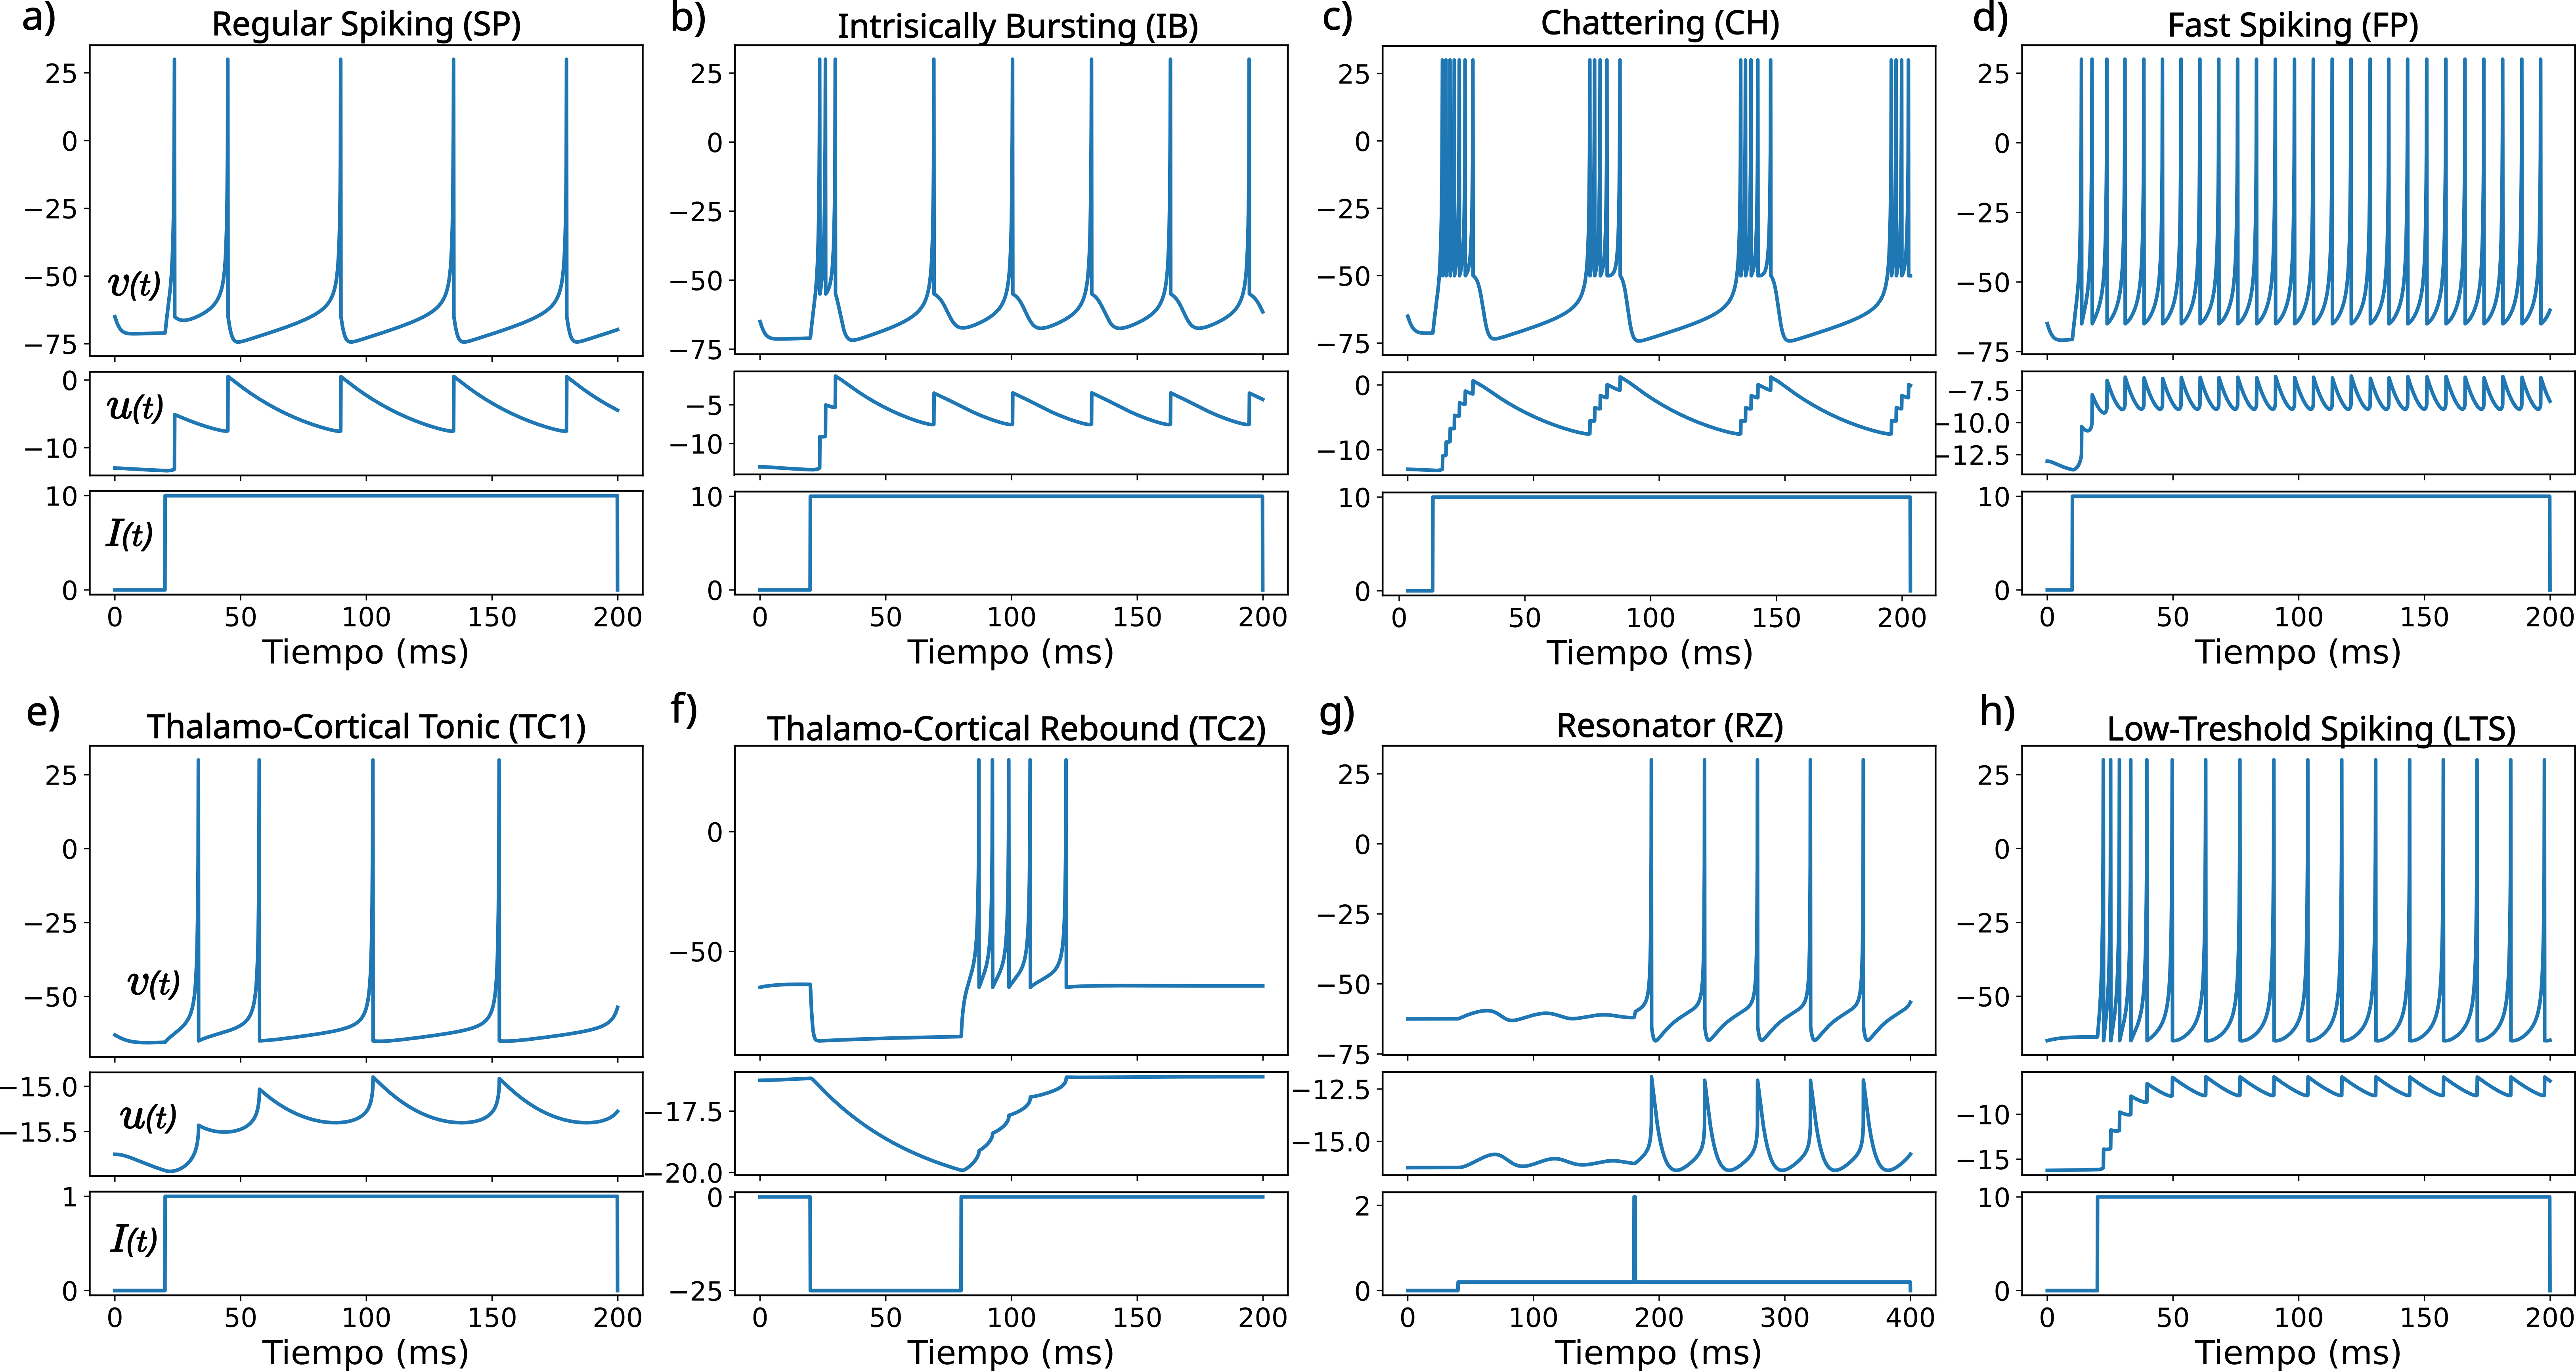
\includegraphics[width=0.85\linewidth]{figs/fig2.png}
    \caption{Distintos tipos de dinámicas neuronales que el modelo reproduce. }
    \label{fig:fig2}
\end{figure*}

\section{Discusión}
Los resultados obtenidos confirman que la integración mediante Runge-Kutta 4 (RK4) con un paso temporal $h = 0.1$ ms reproduce adecuadamente la riqueza cualitativa de las dinámicas neuronales reportadas en el artículo original de Izhikevich \cite{izhikevich2003simple}. La combinación de la dinámica continua de las EDOs con la regla de reseteo discreto permite capturar fenómenos complejos como la adaptación de frecuencia en células RS, el agrupamiento en ráfagas en IB y CH, y el disparo por rebote tras hiperpolarización en TC2.
Desde la perspectiva del análisis numérico, el método RK4 brinda una elevada precisión para la fase continua del potencial de membrana entre disparos. Sin embargo, la condición de reseteo introduce una discontinuidad no suave en el sistema. Como el instante exacto en que $v\small(t)$ cruza los 30 mV rara vez coincide de forma con bajo error con los nodos discretos del paso h, el valor de v en el instante de disparo puede sobrepasar no tan ligeramente la cota antes de ser reseteado. La elección de h = 0.01ms (o menor) resulta un mejor compromiso óptimo entre costo computacional y precisión, evitando desviaciones significativas en la frecuencia de disparo sin requerir esquemas de interpolación de eventos más complejos. 
La diferencia entre la aproximación numérica antes de cruzar el umbral y el paso siguiente, que cruza el umbral, puede ser alta, alrededor de 5-20mV. Esto deja en la figura \ref{fig:fig3} un efecto visible. Lo que se hace en los otros gráficos es al  paso que cruza el umbral remplazarlo por el umbral. \textit{Triggerers} son aquellas aproximaciones que usualmente serian remplazadas con 30mV, el umbral.

\begin{figure}[H]
    \centering
    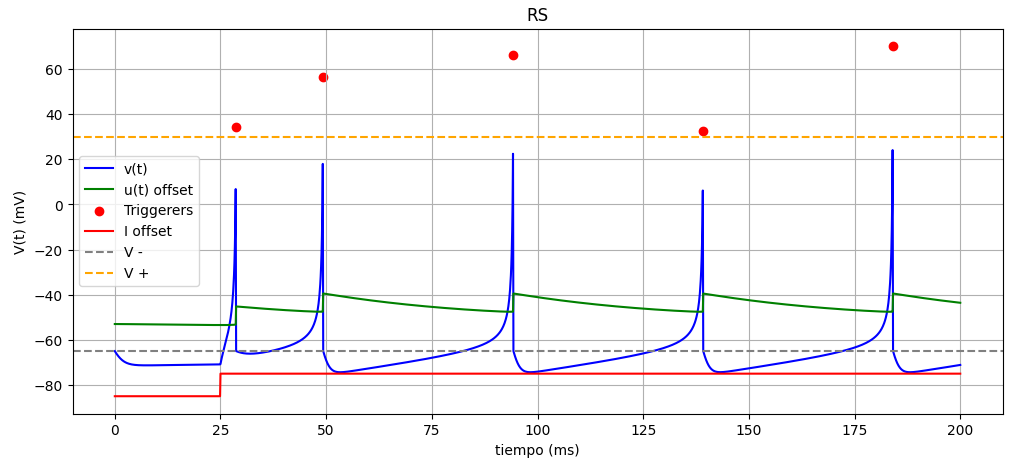
\includegraphics[width=0.48\textwidth]{jumpyAproxTriggerers.png}
        \caption{h=0.1 , 460ms tiempo de computo (i7-10610U)}
    \label{fig:fig3}
\end{figure}

\begin{figure}[H]
    \centering
    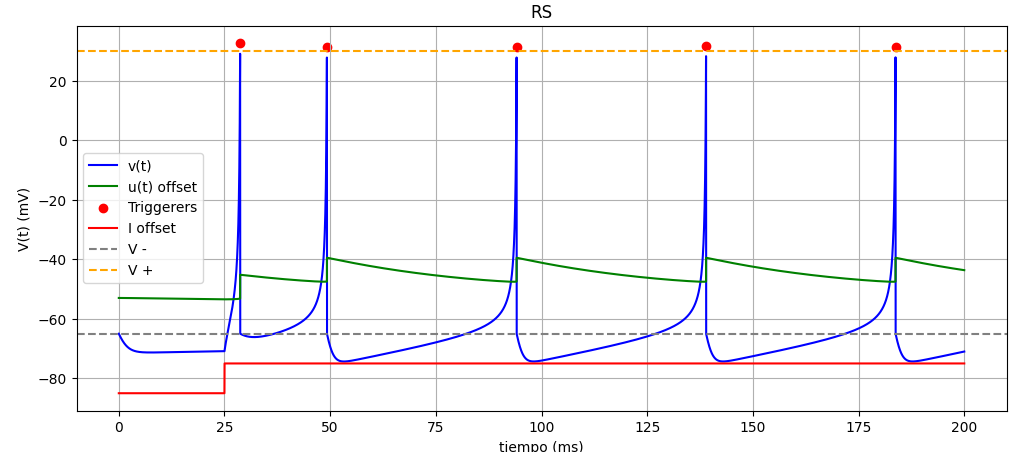
\includegraphics[width=0.48\textwidth]{lessJumpy.png}
    \caption{h=0.01 , 1136ms tiempo de computo (i7-10610U)}
    \label{fig:fig4}
\end{figure}



\bibliography{ref}

\onecolumngrid

\appendix

\section{Parámetros de sistema dinámico}
El modelo de Izhikevich se obtiene reduciendo el modelo de Hodgkin-Huxley mediante análisis de bifurcación y forma normal, condensando la dinámica de canales iónicos en un sistema de dos ecuaciones y cuatro parámetros que, con la eficiencia computacional de un integrate-and-fire, reproduce todo el repertorio de patrones de disparo y estallido observados en neuronas corticales \cite{izhikevich2007dynamical}. A pesar de resultar ser más sencillo puede reproducir dinámicas de distintos tipos de neuronas. Los distintos comportamientos se logran asignando valores a parámetros del sistema dinámico, ademas de diseñar una señal de entrada ($I(t)$) y  configurar valores iniciales de manera especifica. La tabla \ref{tab:parametros_izhikevich} resume los parámetros del sistema dinámico utilizado para cada tipo de neurona de la figura \ref{fig:fig2} .



\begin{table}[ht]
    \centering
    \begin{tabular}{lcccc}
    \hline \hline
    Caso & $a$ & $b$ & $c$ & $d$ \\
    \hline
    RS  & 0.02 & 0.2  & -65 & 8 \\
    IB  & 0.02 & 0.2  & -55 & 4 \\
    CH  & 0.02 & 0.2  & -50 & 2 \\
    FS  & 0.1  & 0.2  & -65 & 2 \\
    TC1 & 0.02 & 0.25 & -65 & 0.05 \\
    TC2 & 0.02 & 0.25 & -65 & 0.05 \\
    RZ  & 0.1  & 0.26 & -65 & 2 \\
    LTS & 0.02 & 0.25 & -65 & 2 \\
    \hline
    \end{tabular}
    \caption{Parámetros del modelo de Izhikevich para distintos comportamientos neuronales.}
    \label{tab:parametros_izhikevich}
\end{table}



Para los tipos RS, IB, CH, FS y LTS se utilizó un escalón de corriente para la corriente de entrada:
\begin{equation}
    I_1(t) =
    \begin{cases} 
        0, & t < 20\text{ ms,} \\ 
        10, & t \geq 20\text{ ms.} 
    \end{cases}
\end{equation}
además de los valores iniciales: $v(0) = -65\text{ mV}$ y $u(0) = b \cdot v(0)$.

Para los paneles TC (1 y 2) y RZ, de la la figura \ref{fig:fig2} se utilizó los siguientes protocolos:

\begin{description}
    \item[TC1 (disparo tónico desde un estado de reposo):] se tomó $v(0) = -63\text{ mV}$, $u(0) = b \cdot v(0)$ y
    \begin{equation}
        I_2(t) =
        \begin{cases} 
            0, & t < 20\text{ ms,} \\ 
            1, & t \geq 20\text{ ms.} 
        \end{cases}
    \end{equation}

    \item[TC2 (\textit{rebound burst} luego de hiperpolarización):] se tomó $v(0) = -65\text{ mV}$, $u(0) = b \cdot v(0)$ y
    \begin{equation}
        I_3(t) =
        \begin{cases} 
            0, & t < 20\text{ ms,} \\ 
            -25, & 20\text{ ms} \leq t < 80\text{ ms,} \\ 
            0, & t \geq 80\text{ ms.} 
        \end{cases}
    \end{equation}
    
    \item[RZ (resonador):] se asignó $v(0) = -62{,}5\text{ mV}$, $u(0) = b \cdot v(0)$ y
    \begin{equation}
        I_4(t) =
        \begin{cases} 
            0, & t < 40\text{ ms,} \\ 
            0{,}2, & 40\text{ ms} \leq t < 180\text{ ms,} \\ 
            2{,}2, & 180\text{ ms} \leq t < 181\text{ ms,} \\ 
            0{,}2, & t \geq 181\text{ ms.} 
        \end{cases}
    \end{equation}
\end{description}

\end{document}
